\marginpar{\href{https://youtu.be/C_W1adH-NVE}{Video}}


$X_1,\ldots,X_n \sim Ber(p)$, iid, p is unknown
\vspace{1cm}
$$\hat{p}=\bar{x}_n = \frac{1}{n} \sum_{i=1}^n X_i$$
\\
$$\frac{\sqrt{n}(\bar{X}_n-p)}{\sqrt{p(1-p)}}$$

\begin{figure}[!ht]
\centering
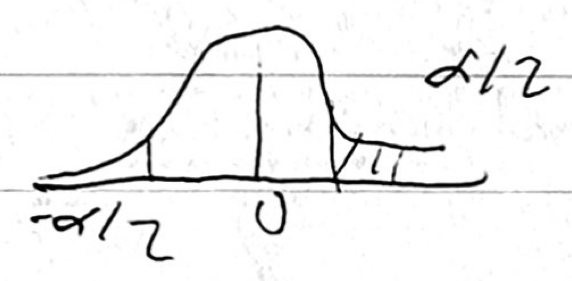
\includegraphics[width=5cm, height=4cm]{IMG_1447.jpeg}
\caption{Guassian Normal}
\end{figure}

$$\sqrt{\frac{p(1-p)}{n}}=\sigma$$

Convention to move denominator to top
$$\frac{x}{\sqrt{a/b}}= \frac{\sqrt{b}x}{\sqrt{a}}$$

\subsection{Hoeffding's inequality}

\marginpar{\href{https://youtu.be/C_W1adH-NVE?t=13m15s}{(13:15)}}

\begin{itemize}
\item one of the most useful inequalities
\item tells about bounded random variables
\item Bernouilli RV's bounded between [0,1]
\end{itemize}


\begin{figure}[!ht]
\centering
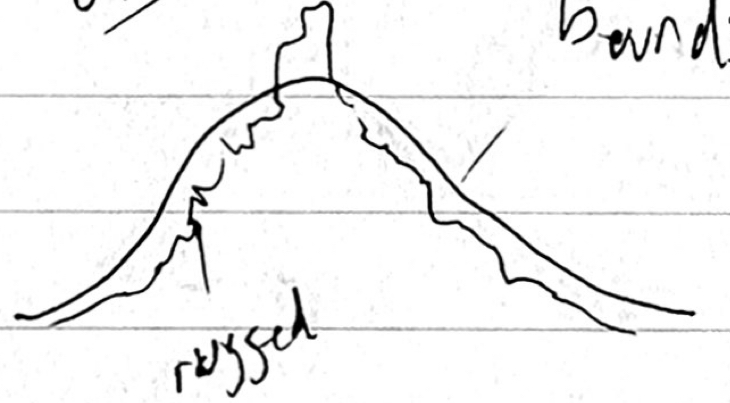
\includegraphics[width=5cm, height=4cm]{IMG_1448.jpeg}
\caption{Bounds Bernoulli (sort of)}
\end{figure}

$$P(|\bar{X}_n - \mu| \le 2e^\frac{-2ne^2}{(b-a)^2}$$
No limits are needed.
\marginpar{\href{https://youtu.be/C_W1adH-NVE?t=22m}{(22:00)}}

Consequences - see slides\\


\marginpar{\href{https://youtu.be/C_W1adH-NVE?t=24m}{(24:00)}}

In statistics the only convergence we care about is the convergence in distribution. (e.g. the one from the CLT - weakest one you could make - good because it will happen more often)

\marginpar{\href{https://youtu.be/C_W1adH-NVE?t27m}{(27:00)}}

Review different types of Convergence.  Ways in which RV's can converge.

\marginpar{\href{https://youtu.be/C_W1adH-NVE?t=27m20s}{(27:20)}}

An RV is something you measure on something that is random.

\marginpar{\href{https://youtu.be/C_W1adH-NVE?t=27m30s}{(27:30)}}
$\omega$ is the snowball.  The thing on which you make your measurements.  Put a ball of snow in the sun for some time then measure volume, inner temperature, surface area; all RV's.  The RV's are a function of the omegas.  This function has to be measurable.

Almost surely (a.s.) convergence


Convergence in probability

\marginpar{\href{https://youtu.be/C_W1adH-NVE?t=3-m}{(30:00)}}
Convergence in $L^p, p \ge 1$.  Extends to vectors

\marginpar{\href{https://youtu.be/C_W1adH-NVE?t=34m}{(34:00)}}
Characteristic function

\marginpar{\href{https://youtu.be/C_W1adH-NVE?t=34m45s}{(34:45)}}
The most common way to prove CLT use the third element??

\marginpar{\href{https://youtu.be/C_W1adH-NVE?t=36m}{(36:00)}}
Types of convergence - 4\\
\marginpar{\href{https://youtu.be/C_W1adH-NVE?t=42m54s}{(42:55)}} cdf's aren't defined for vectors

Wasserman Chapter 5 covers RV convergence.

\subsection{Example (1)[slide]}

\marginpar{\href{https://youtu.be/C_W1adH-NVE?t=43m}{(43:00)}}

You observe the times between arrivals of the T subway at Kendall: $T_1,\ldots,T_n$.  Assume times are:

\begin{itemize}
    \item mutually independent
    \item Exponential RVs with common parameter $\lambda>0$
\end{itemize}

Want to estimate $\lambda$ based on observed arrival times

\subsection{Delta Method (slide)}

\marginpar{\href{https://youtu.be/C_W1adH-NVE?t5820s}{(58:20)}}

\begin{itemize}
    \item LLN - Law of Large Numbers used
    \item First order Tayler expansion
\end{itemize}

\subsection{Slutsky's Theorem}


\marginpar{\href{https://youtu.be/C_W1adH-NVE?t=1h3m15s}{(1:03:35)}}

